\documentclass[11pt]{article}
\usepackage[margin=1in]{geometry}
\usepackage[utf8]{inputenc}
\usepackage[T1]{fontenc}
\usepackage[colorlinks=true,linkcolor=black,citecolor=blue!50!black,urlcolor=blue!50!black]{hyperref}
\usepackage{amsmath,amssymb,amsthm}
\usepackage{microtype}
\usepackage{xcolor}
\usepackage{tikz}
\usetikzlibrary{arrows.meta,positioning,calc}

\newtheorem{proposition}{Proposition}
\newtheorem{lemma}{Lemma}
\theoremstyle{definition}
\newtheorem{assumption}{Assumption}

\newcommand{\KL}{\mathrm{KL}}
\newcommand{\Prn}{\Pr\nolimits_{k+1}}
\newcommand{\fn}{f_{\mathrm{new}}}
\newcommand{\pn}{\pi_{\mathrm{new}}}
\newcommand{\dE}{\Delta E}
\newcommand{\dP}{\Delta P}
\newcommand{\rng}{\operatorname{rng}}
\newcommand{\why}[1]{\tag*{\small(#1)}}

\title{The Return of an Agent That Acts on a Memory:\\ from the four terms to an algorithm, in four steps}
\author{}
\date{Research note, 24 November 2026}

\begin{document}
\maketitle

\paragraph{Question.} An agent has a state-update function $f$ that turns its history into a memory $M_t$, a critic, and a policy that reads only the memory. It learns all three (Figure~\ref{fig:agent}). Learning proceeds in rounds: during a round $f$ and the policy are fixed while the agent collects experience, and between two rounds both change. How should $f$ be trained, and how should the policy change, from one round to the next?

\paragraph{Three things the answer is written in.} The \emph{visible value} $X$ of a memory is the largest action value at each memory value, averaged over the agent's experience and summed over time \eqref{eq:X}; it is what a critic that reads this memory can show. The \emph{hidden loss} of a memory is what is lost when all histories with the same memory value have to take the same action \eqref{eq:loss}. The \emph{four terms} of the state defect measure what the history tells, beyond the memory, about the next observation ($D^0$), about the action just taken once the next observation is seen ($\dE$), about the next action ($\dP$), and about the next observation once the next action is known ($D^+$).

\paragraph{Answer, in four steps.} Round $k$ has $f_k$ and $\pi_k$; between two rounds, training turns $f_k$ into a candidate $\fn$.
\begin{enumerate}
\item If the policy moves a step of size $\alpha$ towards the best actions on the memory of $\fn$, then $J(\pi_{k+1})-J(\pi_k)=\alpha\,\big[X(\fn)-\bar V\big]$ up to a term of order $\alpha^2$, where $\bar V$ is the average value of $\pi_k$ and does not depend on $\fn$ (Proposition~\ref{prop:step}).
\item $X(\fn)$ is the visible value of the whole history minus the hidden loss of the memory of $\fn$ (Proposition~\ref{prop:hide}).
\item For the memory that the policy reads, that of $f_k$, the hidden loss is at most a sum of square roots of the four terms, each times a range of values; for $D^0$ and $\dE$ the terms are those of later times, and they come with a factor that grows when an action is rare (Proposition~\ref{prop:terms}). For a candidate that the policy does not read yet, no bound is proved.
\item So: train candidates on the four terms as auxiliary prediction losses, keep the candidate with the largest visible value as estimated by the critic, and move the policy a small step (Section~\ref{sec:algo}).
\end{enumerate}
Step 2 is exact, and step 1 is exact to first order in $\alpha$. Step 3 is an upper bound, so the theory does not give the weights of the four losses; step 4 tries a few settings of the weights and lets the visible value choose.

\section{Setting}

\begin{figure}[h]
\centering
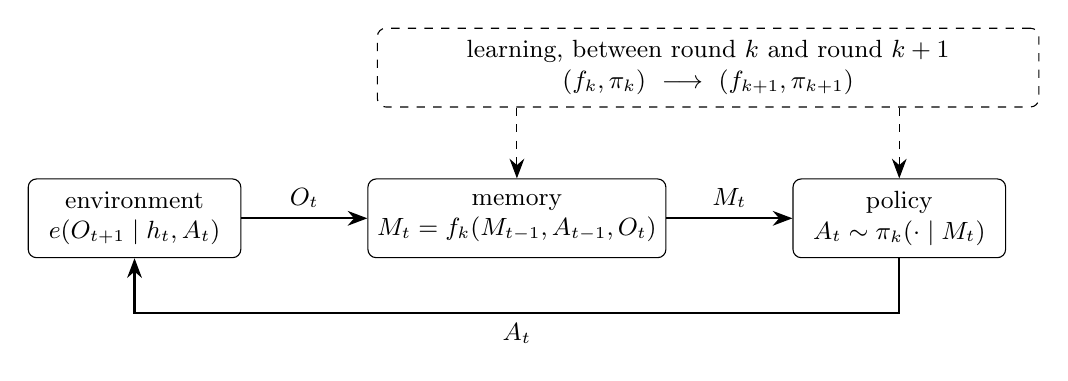
\begin{tikzpicture}[>={Stealth[length=2.5mm]}, node distance=10mm and 16mm,
  box/.style={draw, rounded corners=3pt, minimum height=10mm, minimum width=27mm, align=center, font=\small}]
\node[box] (world) {environment\\ $e(O_{t+1}\mid h_t, A_t)$};
\node[box, right=of world] (mem) {memory\\ $M_t = f_k(M_{t-1}, A_{t-1}, O_t)$};
\node[box, right=of mem] (pol) {policy\\ $A_t \sim \pi_k(\cdot \mid M_t)$};
\draw[->, thick] (world) -- node[above, font=\small] {$O_t$} (mem);
\draw[->, thick] (mem) -- node[above, font=\small] {$M_t$} (pol);
\draw[->, thick] (pol.south) -- ++(0,-7mm) -| node[pos=0.25, below, font=\small] {$A_t$} (world.south);
\node[box, dashed, minimum width=84mm, above=9mm of $(mem.north)!0.5!(pol.north)$] (learn) {learning, between round $k$ and round $k+1$\\ $(f_k,\pi_k)\ \longrightarrow\ (f_{k+1},\pi_{k+1})$};
\draw[->, dashed] (learn.south -| mem.north) -- (mem.north);
\draw[->, dashed] (learn.south -| pol.north) -- (pol.north);
\end{tikzpicture}
\caption{The agent. Solid: one round, in which $f_k$ and $\pi_k$ are fixed and only the memory $M_t$ changes. Dashed: between two rounds, learning changes both. The action depends on the history only through the memory.}\label{fig:agent}
\end{figure}

\paragraph{What is fixed and what is learned.} Learning proceeds in rounds $k=1,2,\dots$ A round is a number of runs of length $T$, all with the same state-update function $f_k$ and the same policy $\pi_k$. Between two rounds learning changes both.
\begin{center}
\small
\begin{tabular}{lll}
\hline
 & during round $k$ & between rounds $k$ and $k+1$\\
\hline
memory $M_t$ & updated at every $t$ by $f_k$ & \\
state-update function & fixed, $f_k$ & learned: gradient steps on prediction losses\\
critic & estimates the values of $\pi_k$ & estimates those of $\pi_{k+1}$\\
policy & fixed, $\pi_k$ & learned: a small step to better actions\\
\hline
\end{tabular}
\end{center}
For fixed $(f_k,\pi_k)$ this is a bounded agent as defined by Abel et al.\ (2023a), with $f_k$ as their state-update function; their agent state holds everything the agent keeps, parameters included, while here $M_t$ is the memory alone and the parameters change between rounds. In the words of Abel et al.\ (2023b), each pair $(f,\pi)$ is a base agent, and learning selects the base agent of the next round.

The history is $h_t=(O_1,A_1,\dots,A_{t-1},O_t)$, and $h$ denotes a value of $h_t$. An observation $o$ contains a reward $r(o)$. All sets are finite, actions are taken at $t=1,\dots,T-1$, and $\gamma\in[0,1]$. All probabilities and values below are those of the agent of round $k$, and sums over values of a memory or of an observation run over the values that have positive probability.

\begin{assumption}[Environment]\label{as:env}
$O_1$ has a fixed law and $O_{t+1}\sim e(\cdot\mid h_t,A_t)$. The environment may depend on the whole history.
\end{assumption}
\begin{assumption}[Memory]\label{as:mem}
$M_1$ is computed from $O_1$ by $f_k$, and $M_t=f_k(M_{t-1},A_{t-1},O_t)$ for $t\ge2$. The memory contains the time $t$, so values of the memory at different times are different. $m$ is a value of $M_t$, and $m'=f_k(m,a,o)$ is the next value after the action $a$ and the observation $o$. We also write $f_k(h_t)$ for $M_t$, the memory that $f_k$ computes from the history, and likewise for any other state-update function.
\end{assumption}
\begin{assumption}[Policy]\label{as:pol}
The agent takes $A_t=a$ after $h_t$ with probability $\pi_k(a\mid M_t)>0$. Where the agent explores, the exploration is part of $\pi_k$.
\end{assumption}

$\Pr$ is the law of the experience under $\pi_k$, and $J(\pi_k)$ is the expectation of $\sum_{t=1}^{T-1}\gamma^{t-1}r(O_{t+1})$. For every history and action,
\begin{equation}\label{eq:bellman}
Q_t(h,a)=\sum_oe(o\mid h,a)\big[r(o)+\gamma V_{t+1}(h,a,o)\big],\qquad V_t(h)=\sum_a\pi_k(a\mid m)\,Q_t(h,a),\qquad V_T=0,
\end{equation}
where $(h,a,o)$ is the next history and $m$ the memory value of $h$. The \emph{average value} of $\pi_k$ is
\begin{equation}\label{eq:Vbar}
\bar V=\sum_{t=1}^{T-1}\gamma^{t-1}\sum_h\Pr(h_t=h)\,V_t(h).
\end{equation}
It is not $J(\pi_k)$, which is its first term.

\paragraph{A candidate and its visible value.} Let $\fn$ be what training produces between the two rounds: $f_k$ after some gradient steps. $\fn(h_t)$ is the memory that it computes from the same history, and $n$ is one of its values; it also contains the time. The policy still reads $M_t$. We say that $\fn$ is \emph{finer} than $f_k$ when $M_t$ is a function of $\fn(h_t)$; a candidate need not be finer. With $\Pr(h\mid n)$ the probability of $h_t=h$ given $\fn(h_t)=n$, the values on the memory of $\fn$ average those of the histories,
\[
Q_t(n,a)=\sum_h\Pr(h\mid n)\,Q_t(h,a),\qquad V_t(n)=\sum_h\Pr(h\mid n)\,V_t(h),
\]
and the \emph{visible value} of this memory is
\begin{equation}\label{eq:X}
X(\fn)=\sum_{t=1}^{T-1}\gamma^{t-1}\sum_n\Pr(\fn(h_t)=n)\,\max_aQ_t(n,a).
\end{equation}
With $f_k$ in the place of $\fn$ these are $Q_t(m,a)$ and $V_t(m)$, and they are what the critic of an actor-critic agent learns: the average return after $M_t=m$ and $A_t=a$ is $\sum_h\Pr(h\mid m,a)\,Q_t(h,a)$, and $\Pr(h\mid m,a)=\Pr(h\mid m)$ because $\pi_k$ reads $m$ alone. So $X(f_k)$ is the average of the critic's largest action value. The history is the memory of a state-update function that forgets nothing; its visible value, written $X(h)$, has $\max_aQ_t(h,a)$ in \eqref{eq:X}.

The weights $\Pr(h\mid n)$ do not depend on the action. So $Q_t(n,a)$ is the average return after the action $a$ at $n$ when the action is drawn independently of the history, for instance uniformly. Unless $\fn$ is finer than $f_k$, it is in general not the average return after $a$ at $n$ when the action is drawn by $\pi_k$, which reads another memory. With actions drawn by $\pi_k$, each step has to be weighted by $1/\pi_k(A_t\mid M_t)$: the average over the steps with $\fn(h_t)=n$ of the return times $\mathbf 1\{A_t=a\}/\pi_k(a\mid M_t)$ is $\sum_h\Pr(h\mid n)\,\pi_k(a\mid m)\,Q_t(h,a)/\pi_k(a\mid m)=Q_t(n,a)$.

\paragraph{Example.} $T=3$, $\gamma=1$, two actions. $O_1$ is a fair bit $c$. If $A_1=c$, then $O_2$ shows a fair bit $d$; otherwise $O_2$ is blank. The bit $d$ is drawn whether or not it is shown. The only reward is in $O_3$: it is $1$ if $A_2=d$ and $0$ otherwise. The memory of $f_k$ is empty at time $1$, so it forgets $c$, and it is $O_2$ at time $2$. The policy $\pi_k$ is uniform, and $J(\pi_k)=\tfrac12$.

\section{Step 1: what a small policy step gains}

This step is the learning of the policy, from $\pi_k$ to $\pi_{k+1}$, for a given candidate $\fn$. Let $\pn$ read the memory of $\fn$ and take, at each memory value $n$, an action with the largest $Q_t(n,a)$; when several actions are largest, $\pn$ takes them in proportion to $\Pr(A_t=a\mid\fn(h_t)=n)$. The agent moves to
\[
\pi_{k+1}=(1-\alpha)\,\pi_k+\alpha\,\pn,\qquad0<\alpha\le1 .
\]
This policy reads both memories, so the agent of round $k+1$ keeps both: $f_{k+1}$ computes the pair $(M_t,\fn(h_t))$. When $\alpha=1$, or when $\fn$ is finer than $f_k$, $f_{k+1}$ is $\fn$ alone. For $\alpha<1$ the new policy again takes every action. Write
\begin{equation}\label{eq:g}
g_t(h)=\sum_a\big[\pn(a\mid n)-\pi_k(a\mid m)\big]\,Q_t(h,a),
\end{equation}
with $m$ and $n$ the memory values of $h$ under $f_k$ and $\fn$. Let $\kappa$ be the largest value of $\sum_a\pn(a\mid n)^2/\pi_k(a\mid m)-1$ over the histories $h_t$ of positive probability with $t\le T-2$; it is a chi-square distance between $\pn$ and $\pi_k$ at one history.

\begin{lemma}[Known: performance difference; Kakade and Langford, 2002]\label{lem:pdl}
For every agent $\lambda(a\mid h)$, with $\Pr_\lambda$ its law,
\[
J(\lambda)-J(\pi_k)=\sum_{t=1}^{T-1}\gamma^{t-1}\sum_h\Pr\nolimits_\lambda(h_t=h)\sum_a\big[\lambda(a\mid h)-\pi_k(a\mid m)\big]\,Q_t(h,a).
\]
\end{lemma}

\begin{proposition}[A step towards a memory]\label{prop:step}
Under Assumptions~\ref{as:env} to~\ref{as:pol}:

(a) $\displaystyle\sum_{t=1}^{T-1}\gamma^{t-1}\sum_h\Pr(h_t=h)\,g_t(h)=X(\fn)-\bar V$, and $\bar V$ does not depend on $\fn$.

(b) With $s_t$ the standard deviation of $g_t(h_t)$ under $\pi_k$,
\[
\Big|J(\pi_{k+1})-J(\pi_k)-\alpha\big[X(\fn)-\bar V\big]\Big|\le\alpha\sum_{t=2}^{T-1}\gamma^{t-1}\sqrt{(1+\alpha^2\kappa)^{t-1}-1}\;s_t ,
\]
and $\sqrt{(1+\alpha^2\kappa)^{t-1}-1}\le\alpha\sqrt{(t-1)\kappa}\,(1+\alpha^2\kappa)^{(t-2)/2}$.
\end{proposition}
\begin{proof}
(a) Group the histories by $n$:
\[
\sum_h\Pr(h_t=h)\sum_a\pn(a\mid n)\,Q_t(h,a)=\sum_n\Pr(\fn(h_t)=n)\sum_a\pn(a\mid n)\,Q_t(n,a),
\]
and $\pn$ takes maximizing actions by a rule that depends on $n$ alone. The other part of $g_t$ is $-V_t(h)$, and its sum is $-\bar V$ by \eqref{eq:Vbar}.

(b) By Lemma~\ref{lem:pdl} with $\lambda=\pi_{k+1}$, $J(\pi_{k+1})-J(\pi_k)=\alpha\sum_t\gamma^{t-1}\sum_h\Prn(h_t=h)\,g_t(h)$. where $\Prn$ is the law of the experience under $\pi_{k+1}$. Let $L_t(h)=\Prn(h_t=h)/\Pr(h_t=h)$, which is the product over the times $\tau<t$ of $\pi_{k+1}(a_\tau\mid h_\tau)/\pi_k(a_\tau\mid m_\tau)$, with $a_\tau$, $h_\tau$, $m_\tau$ the action, the history and the memory value at time $\tau$ along $h$; and let $\bar g_t$ be the mean of $g_t(h_t)$ under $\pi_k$. Since $\sum_h\Pr(h_t=h)\big[L_t(h)-1\big]=0$,
\begin{align*}
\Big|\sum_h\big[\Prn(h_t=h)-\Pr(h_t=h)\big]g_t(h)\Big|&=\Big|\sum_h\Pr(h_t=h)\big[L_t(h)-1\big]\big[g_t(h)-\bar g_t\big]\Big|\\
&\le\sqrt{\sum_h\Pr(h_t=h)\,L_t(h)^2-1}\;s_t \why{Cauchy--Schwarz}.
\end{align*}
Summing first over the last action and observation of $h$, and using $\sum_a\pi_{k+1}(a\mid h)^2/\pi_k(a\mid m)=1+\alpha^2\big[\sum_a\pn(a\mid n)^2/\pi_k(a\mid m)-1\big]\le1+\alpha^2\kappa$,
\[
\sum_h\Pr(h_t=h)\,L_t(h)^2\le(1+\alpha^2\kappa)\sum_h\Pr(h_{t-1}=h)\,L_{t-1}(h)^2,
\]
and $L_1=1$, so the term $t=1$ vanishes. The last claim is $(1+z)^p-1\le pz(1+z)^{p-1}$ for $z\ge0$ and an integer $p\ge1$.
\end{proof}

So $J(\pi_{k+1})-J(\pi_k)$ is $\alpha\,[X(\fn)-\bar V]$ up to the right side of (b), which is of order $\alpha^2$, and the candidate enters the first-order part only through its visible value. The step is a gain when $\alpha\,[X(\fn)-\bar V]$ exceeds the right side of (b); so when $X(\fn)>\bar V$ it is a gain for every small enough $\alpha$, and it need not be one for $\alpha=1$. For every $\fn$ finer than $f_k$ we have $X(\fn)\ge X(f_k)\ge\bar V$: the first inequality is Step~2, and the second holds because a largest value is at least an average. Between two candidates, the one with the larger visible value gives the larger gain once $\alpha$ times the difference of the two visible values exceeds the sum of their two right sides of (b). With $\fn=f_k$ this is the usual small policy step on the current memory.

\paragraph{In the example.} Take $\fn=f_k$. At time $1$ both actions have the value $\tfrac12$. At time $2$ the largest value is $1$ when $d$ is shown, which has probability $\tfrac12$, and $\tfrac12$ otherwise. So $X(f_k)=\tfrac12+\tfrac34=\tfrac54$, while $\bar V=\tfrac12+\tfrac12=1$, and $X(f_k)-\bar V=\tfrac14$. At time $1$ the two actions tie, so $\pn=\pi_k$ there, the visits at time $2$ do not change, and the left side of (b) is zero. The policy step with $\alpha=1$ gives $J=\tfrac34$. (After it the policy at time $2$ no longer takes every action; nothing below needs that it does.)

\section{Step 2: what a memory hides}

In this step the policy is fixed and nothing is learned: it compares what two state-update functions show of the values of the same agent. The \emph{hidden loss} at a memory value $n$ of $\fn$ is the value when each history with this memory value takes its own best action, minus the value when all of them take the one action that is best on average:
\begin{equation}\label{eq:loss}
\sum_h\Pr(h\mid n)\,\max_aQ_t(h,a)-\max_aQ_t(n,a).
\end{equation}

\begin{proposition}[Visible value and hidden loss]\label{prop:hide}
The visible value of the history minus that of the memory of $\fn$ is the average hidden loss,
\[
X(h)-X(\fn)=\sum_{t=1}^{T-1}\gamma^{t-1}\sum_n\Pr(\fn(h_t)=n)\,\big[\text{hidden loss \eqref{eq:loss} at }n\big]\ \ge0 .
\]
If $\fn$ is finer than $f_k$, then $X(\fn)\ge X(f_k)$.
\end{proposition}
\begin{proof}
Group the histories by $n$ in $X(h)$. Each hidden loss is nonnegative because $Q_t(n,a)$ is an average of $Q_t(h,a)$, and the maximum of an average is at most the average of the maxima. For the last claim, $Q_t(m,a)$ is an average of the $Q_t(n,a)$ over the values $n$ that give the memory value $m$, and the same argument applies with the memory of $\fn$ in the role of the history.
\end{proof}

So training $f$ does not by itself change the return. It changes how much of $X(h)$, the most that any memory can show, the critic can see; the return moves when the policy then takes its step (Step~1).

\paragraph{In the example.} With the uniform policy, $Q_1(h,a)=\tfrac12$ for both values of $c$ and both actions: the hidden loss of the memory of $f_k$ at time $1$ is $0$, and keeping $c$ adds nothing to the visible value. Now take the next round, after the policy step with $\alpha=1$. There $Q_1(h,a)$ is $1$ if $a=c$ and $\tfrac12$ otherwise, while on the memory of $f_k$ both actions have the value $\tfrac34$: the hidden loss at time $1$ is $1-\tfrac34=\tfrac14$. A candidate that keeps $c$ at time $1$, and still $O_2$ at time $2$, has a visible value larger by $\tfrac14$. What a memory hides depends on the current policy.

\section{Step 3: the hidden loss and the four terms}

This step is for the memory of $f_k$, which the policy reads; again nothing is learned inside it. Below, $a$ and $b$ are actions at time $t$ and $a'$ is the action at time $t+1$. Conditional laws such as $\Pr(o\mid m,b,a')$ or $\Pr(a\mid m,o)$ are those of the experience under $\pi_k$ given the stated values. Let $\Pr(o\mid m,a)=\sum_h\Pr(h\mid m)\,e(o\mid h,a)$. The state defect and its four terms are
\begin{align*}
D_t(m,a)&=I(h_t;O_{t+1}\mid M_t=m,A_t=a)=\sum_h\Pr(h\mid m)\,\KL\big(e(\cdot\mid h,a)\,\big\|\,\Pr(\cdot\mid m,a)\big),\\
D^0_t(m)&=I(h_t;O_{t+1}\mid M_t=m),\\
\dE_t(m)&=I(h_t;A_t\mid M_t=m,O_{t+1}),\\
\dP_t(m,a)&=I(h_t;A_{t+1}\mid M_t=m,A_t=a),\\
D^+_t(m,a)&=I(h_t;O_{t+1}\mid M_t=m,A_t=a,A_{t+1}),
\end{align*}
the last two for $t\le T-2$. The chain rule gives two splits of the state defect. The split at the current action is $\sum_a\pi_k(a\mid m)D_t(m,a)=D^0_t(m)+\dE_t(m)$, since $I(h_t;A_t\mid M_t=m)=0$. The split at the next action is $D_t(m,a)=\dP_t(m,a)+D^+_t(m,a)$ for $t\le T-2$, since given $(m,a,O_{t+1})$ the next action depends on $M_{t+1}$ alone. Both reasons use that the policy reads this memory.

\begin{lemma}[One step]\label{lem:onestep}
For every history $h$ with memory value $m$ and every action $a$,
\begin{align}
Q_t(h,a)-Q_t(m,a)={}&\sum_o\big[e(o\mid h,a)-\Pr(o\mid m,a)\big]\big[r(o)+\gamma V_{t+1}(m')\big] \label{eq:now}\\
&+\gamma\big[u_t(h,a)-\bar u_t(m,a)\big], \nonumber
\end{align}
where $u_t(h,a)=\sum_oe(o\mid h,a)\big[V_{t+1}(h,a,o)-V_{t+1}(m')\big]$ and $\bar u_t(m,a)$ is its average over $h$ with the weights $\Pr(h\mid m)$.
\end{lemma}
\begin{proof}
Add and subtract $\gamma V_{t+1}(m')$ in the bracket of \eqref{eq:bellman}; then average over $h$ with the weights $\Pr(h\mid m)$, and subtract.
\end{proof}

The sum \eqref{eq:now} is the part of the difference that is made at time $t$: the two predictions of the next observation, from the history and from the memory, differ, and the difference is weighted by the reward plus the value of the next memory. The other part is carried over from time $t+1$: it is zero when $V_{t+1}(h)=V_{t+1}(m)$ for every next history $h$ with memory value $m$.

\begin{lemma}[Known: Pinsker's inequality; Cover and Thomas, 2006]\label{lem:tool}
For laws $p$, $q$ on a finite set with $q(x)=0\Rightarrow p(x)=0$ and a function $w$: $\big|\sum_x[p(x)-q(x)]w(x)\big|\le\rng_xw(x)\,\sqrt{\tfrac12\KL(p\,\|\,q)}$, where the \emph{range} $\rng_xw(x)$ is $\max_xw(x)-\min_xw(x)$ over the $x$ with $q(x)>0$.
\end{lemma}

Three sizes are used. $\rho_t(m,a)$ is the root of the average of $\big[\eqref{eq:now}\big]^2$ over $h$ with the weights $\Pr(h\mid m)$: the size of the part made at time $t$, for one action. $\rho_t(m)$, without an action, is the same root with $\sum_a\pi_k(a\mid m)\times\eqref{eq:now}$ in the place of \eqref{eq:now}. The size of the carried part is
\[
\nu_t(m,a)=\sqrt{\sum_h\Pr(h\mid m)\sum_oe(o\mid h,a)\big[V_{t+1}(h,a,o)-V_{t+1}(m')\big]^2}\,.
\]

\begin{proposition}[The hidden loss and the four terms]\label{prop:terms}
Let $m$ be a value of the memory of $f_k$ at time $t$ and $a^*$ an action with the largest $Q_t(m,a)$.

(a) The hidden loss \eqref{eq:loss} at $m$ is at most $\displaystyle\frac12\sum_{a\ne a^*}\ \sum_{b\in\{a,a^*\}}\big[\rho_t(m,b)+\gamma\,\nu_t(m,b)\big]$.

(b) The part made at time $t$ is bounded by the state defect of the action, as a whole or split at the next action:
\begin{align*}
\rho_t(m,b)&\le\rng_o\big[r(o)+\gamma V_{t+1}(m')\big]\sqrt{\tfrac12\,D_t(m,b)},\\
\rho_t(m,b)&\le\rng_{a'}\sum_o\Pr(o\mid m,b,a')\big[r(o)+\gamma Q_{t+1}(m',a')\big]\sqrt{\tfrac12\,\dP_t(m,b)}\\
&\quad+\max_{a'}\rng_o\big[r(o)+\gamma Q_{t+1}(m',a')\big]\sqrt{\tfrac12\,D^+_t(m,b)}\qquad(t\le T-2).
\end{align*}

(c) The carried part is bounded by the error of the state value at later times, and this error is bounded with the split at the current action. In each sum over $h$ below, $m$ is the memory value of $h$. For each action $b$, for $1\le i\le T-1$ and $i\le j\le T-1$,
\begin{align*}
\sum_m\Pr(M_t=m)\,\nu_t(m,b)&\le\big[\min_m\pi_k(b\mid m)\big]^{-1/2}\sqrt{\sum_h\Pr(h_{t+1}=h)\big[V_{t+1}(h)-V_{t+1}(m)\big]^2},\\
\sqrt{\sum_h\Pr(h_i=h)\big[V_i(h)-V_i(m)\big]^2}&\le\sum_{j=i}^{T-1}\gamma^{j-i}\sqrt{\sum_m\Pr(M_j=m)\,\rho_j(m)^2},\\
\rho_j(m)&\le\rng_o\bar y(o)\,\sqrt{\tfrac12\,D^0_j(m)}+\max_o\rng_ay_a(o)\,\sqrt{\tfrac12\,\dE_j(m)},
\end{align*}
where $y_a(o)=r(o)+\gamma V_{j+1}(f_k(m,a,o))$ and $\bar y(o)$ is its average over the action with the weights $\Pr(a\mid m,o)$. In (a) the action $a^*$ depends on $m$; there use $\nu_t(m,a^*)\le\sum_b\nu_t(m,b)$.
\end{proposition}
\begin{proof}
(a) Let $x_a(h)=Q_t(h,a)-Q_t(h,a^*)$, with mean $\bar x_a=Q_t(m,a)-Q_t(m,a^*)\le0$ over $h$. The hidden loss is the mean of $\max_a x_a(h)\le\sum_{a\ne a^*}\max\{x_a(h),0\}\le\sum_{a\ne a^*}\max\{x_a(h)-\bar x_a,0\}$, and the mean of the positive part of a variable with mean zero is half the mean of its absolute value. By Lemma~\ref{lem:onestep}, $x_a(h)-\bar x_a$ is \eqref{eq:now} for $a$ minus \eqref{eq:now} for $a^*$ plus $\gamma$ times the same difference of $u_t-\bar u_t$. The mean of an absolute value is at most the root of the mean square; then use Minkowski's inequality, the fact that subtracting $\bar u_t$ does not increase the mean square, and Jensen's inequality for $u_t^2$.

(b) Lemma~\ref{lem:tool} with $p=e(\cdot\mid h,b)$ and $q=\Pr(\cdot\mid m,b)$; square and average over $h$. For the second bound write $V_{t+1}(m')=\sum_{a'}\pi_k(a'\mid m')Q_{t+1}(m',a')$, so that \eqref{eq:now} is a difference of two joint laws of $(A_{t+1},O_{t+1})$. Adding and subtracting the law of $A_{t+1}$ from the history times the law of $O_{t+1}$ given $A_{t+1}$ from the memory splits it into a part with the two laws of $A_{t+1}$ and a part with the two laws of $O_{t+1}$ given $A_{t+1}$. Apply Lemma~\ref{lem:tool} to each, then Minkowski's and Jensen's inequalities; the averages of the divergences are $\dP_t$ and $D^+_t$.

(c) First line: the next history $(h,a,o)$ has probability $\Pr(h_t=h)\pi_k(a\mid m)e(o\mid h,a)$, so the average of $\nu_t(m,a)^2$ over $(M_t,A_t)$ is the sum under the root. Then use Jensen's inequality and $\nu_t(m,b)^2\le\pi_k(b\mid m)^{-1}\sum_a\pi_k(a\mid m)\,\nu_t(m,a)^2$. Second line: average Lemma~\ref{lem:onestep} over the action with $\pi_k(a\mid m)$. By Minkowski's and Jensen's inequalities as in (a), the root on the left at time $i$ is at most $\sqrt{\sum_m\Pr(M_i=m)\rho_i(m)^2}$ plus $\gamma$ times the same root at time $i+1$, and the root at time $T$ is zero. Third line: Bayes' rule gives $\pi_k(a\mid m)\big[e(o\mid h,a)-\Pr(o\mid m,a)\big]=\big[\Pr(o\mid h)-\Pr(o\mid m)\big]\Pr(a\mid m,o)+\Pr(o\mid h)\big[\Pr(a\mid h,o)-\Pr(a\mid m,o)\big]$; sum over $a$ and $o$ against $y_a(o)$, apply Lemma~\ref{lem:tool} to the law of the observation and, for each $o$, to the law of the action, then Minkowski's and Jensen's inequalities. The averages of the divergences are $D^0_j$ and $\dE_j$.
\end{proof}

So the hidden loss of the memory that the policy reads has two sources. First, histories with the same memory value predict the consequences of an action differently. This is bounded with $D_t$ of the two actions that are compared, or, for $t\le T-2$, with their $\dP_t$ and $D^+_t$. Second, the values at the next time are themselves in error. This is bounded with $D^0_j$ and $\dE_j$ at the later times $j$, as a root mean square over the memory values and with a factor that grows as an action becomes rare. Each term comes with its own range of values. These are upper bounds: a term can be large where the hidden loss is zero, for instance when the history knows more about a part of the observation on which no value depends. So the four terms say what $f$ can be trained to predict, and the visible value says whether a change of $f$ helped.

\paragraph{In the example.} Take again the round after the policy step with $\alpha=1$, at time $1$. Here $D_1(m,a)=\ln2$. Split at the current action, $D^0_1=0$ and $\dE_1=\ln2$; split at the next action, $\dP_1=0$ and $D^+_1=\ln2$. The value of the next memory is $1$ when $d$ is shown and $\tfrac12$ otherwise, and \eqref{eq:now} is $\pm\tfrac14$, so $\rho_1(m,a)=\tfrac14\le\tfrac12\sqrt{\ln2/2}\approx0.29$. The carried part is zero because the value at time $2$ depends on $O_2$ alone, and (a) reads $\tfrac14\le\tfrac12\big(\tfrac14+\tfrac14\big)$. In the round before, the four terms are the same, but the range is zero and so is the hidden loss. For a candidate that keeps $c$ at time $1$ the same four formulas give zero.

\section{Step 4: the algorithm}\label{sec:algo}

\paragraph{The four prediction losses.} For a candidate $\fn$, each loss is the average log-loss of a predictor that reads the memory of $\fn$:
\begin{center}
\small
\begin{tabular}{lll}
\hline
term & predict & from\\
\hline
$D^0$ & $O_{t+1}$ & $\fn(h_t)$\\
$\dE$ & $A_t$ & $\fn(h_t)$ and $O_{t+1}$\\
$\dP$ & $A_{t+1}$ & $\fn(h_t)$ and $A_t$\\
$D^+$ & $O_{t+1}$ & $\fn(h_t)$, $A_t$ and $A_{t+1}$\\
\hline
\end{tabular}
\end{center}
For a variable $Y$ and a memory $N$ that is a function of the history, the smallest average log-loss of predicting $Y$ from $N$ is $H(Y\mid N)=I(h_t;Y\mid N)+H(Y\mid h_t)$, and the last entropy does not depend on the candidate; the same holds with the other variables that the predictor reads added to every condition. So the smallest value of each loss is the average of its term, computed with the memory of the candidate, plus a number that does not depend on the candidate.

\begin{center}
\fbox{\begin{minipage}{0.94\linewidth}
\textbf{Round $k$.} The agent makes a number of runs of length $T$ with $f_k$ and $\pi_k$ fixed; $\pi_k$ takes every action with positive probability, as a softmax policy does. Then, from the experience of the round, as in an actor-critic method:
\begin{enumerate}
\item \emph{Candidates.} For each of a few settings of four weights, start from $f_k$ and take gradient steps on the weighted sum of the four prediction losses. These are the auxiliary losses of $f$. Each setting gives one candidate $\fn$, and $f_k$ itself is a candidate too.
\item \emph{Critic.} For $f_k$ this is the usual critic, which learns the return after $(M_t,A_t)$. For every other candidate, train a critic on its memory in the same way, with each step weighted by $1/\pi_k(A_t\mid M_t)$: it learns $Q_t(n,a)$. The visible value is \eqref{eq:X} with the critic's values, and $\bar V$ is \eqref{eq:Vbar} with the returns of the round.
\item \emph{Choice.} Keep the candidate with the largest visible value.
\item \emph{Policy.} If that visible value exceeds $\bar V$, set $\pi_{k+1}=(1-\alpha)\pi_k+\alpha\pn$ with a small $\alpha$, where $\pn$ takes the best actions on the memory of the candidate; $f_{k+1}$ then computes the memories of both $f_k$ and the candidate. Otherwise $\pi_{k+1}=\pi_k$ and $f_{k+1}=f_k$. Go to round $k+1$.
\end{enumerate}
\end{minipage}}
\end{center}

Each line rests on one statement, except the first.
\begin{itemize}\setlength{\itemsep}{0pt}
\item Line 1 is a choice. The hidden loss of the memory that the policy reads is bounded with the four terms (Proposition~\ref{prop:terms}), so they are what $f$ is trained to lower; for a candidate no bound is proved, and lines 2 and 3 check whether the training helped.
\item Line 2 weights each step by $1/\pi_k(A_t\mid M_t)$ because $Q_t(n,a)$ is defined with weights $\Pr(h\mid n)$ that do not depend on the action, while $\pi_k$ chooses its action from another memory. The weights are large where an action is rare.
\item Lines 3 and 4 are Proposition~\ref{prop:step}: the first-order change of the return is $\alpha\,[X(\fn)-\bar V]$, and the step is small because of (b). The loop repeats because what a memory hides changes with the policy.
\end{itemize}

\paragraph{In the example.} Round 1: the candidate is $f_k$ itself, and the policy step gives $J=\tfrac34$. Round 2: a candidate that keeps $c$ has all four terms zero at time $1$ and a visible value larger by $\tfrac14$; the policy step towards it gives $J=1$.

\paragraph{Not covered.}
\begin{itemize}\setlength{\itemsep}{0pt}
\item A bound on the hidden loss of a candidate that the policy does not read yet. Proposition~\ref{prop:terms} and the two splits are for the memory that the policy reads.
\item The weights of the four losses. No statement gives them.
\item How small $\alpha$ has to be. For a large step the ranking of candidates by visible value need not hold.
\item Dropping the memory of $f_k$ after a step with $\alpha<1$, as an agent with one network for $f$ does.
\item Estimation from finitely many runs, a critic that bootstraps, and an agent that changes $f$ and the policy at every time step.
\end{itemize}

\paragraph{Longer version.} Line-by-line proofs of Step~3 are in the folder \texttt{archive}, file\\ {\small\texttt{main\_theory\_to\_algorithm\_paper\_style\_2026-11-24.tex}}.

\begin{thebibliography}{4}
\bibitem[Abel et~al.(2023a)]{abel2023bounded}
D.~Abel, A.~Barreto, H.~van Hasselt, B.~Van~Roy, D.~Precup, and S.~Singh.
\newblock On the convergence of bounded agents.
\newblock arXiv:2307.11044, 2023.

\bibitem[Abel et~al.(2023b)]{abel2023definition}
D.~Abel, A.~Barreto, B.~Van~Roy, D.~Precup, H.~van Hasselt, and S.~Singh.
\newblock A definition of continual reinforcement learning.
\newblock arXiv:2307.11046, 2023.

\bibitem[Cover and Thomas(2006)]{cover2006elements}
T.~M. Cover and J.~A. Thomas.
\newblock \emph{Elements of Information Theory}.
\newblock Wiley, 2nd edition, 2006.

\bibitem[Kakade and Langford(2002)]{kakade2002cpi}
S.~Kakade and J.~Langford.
\newblock Approximately optimal approximate reinforcement learning.
\newblock In \emph{International Conference on Machine Learning (ICML)}, 2002.
\end{thebibliography}

\end{document}
